\documentclass[twoside]{book}

% Packages required by doxygen
\usepackage{fixltx2e}
\usepackage{calc}
\usepackage{doxygen}
\usepackage[export]{adjustbox} % also loads graphicx
\usepackage{graphicx}
\usepackage[utf8]{inputenc}
\usepackage{makeidx}
\usepackage{multicol}
\usepackage{multirow}
\PassOptionsToPackage{warn}{textcomp}
\usepackage{textcomp}
\usepackage[nointegrals]{wasysym}
\usepackage[table]{xcolor}

% Font selection
\usepackage[T1]{fontenc}
\usepackage[scaled=.90]{helvet}
\usepackage{courier}
\usepackage{amssymb}
\usepackage{sectsty}
\renewcommand{\familydefault}{\sfdefault}
\allsectionsfont{%
  \fontseries{bc}\selectfont%
  \color{darkgray}%
}
\renewcommand{\DoxyLabelFont}{%
  \fontseries{bc}\selectfont%
  \color{darkgray}%
}
\newcommand{\+}{\discretionary{\mbox{\scriptsize$\hookleftarrow$}}{}{}}

% Page & text layout
\usepackage{geometry}
\geometry{%
  a4paper,%
  top=2.5cm,%
  bottom=2.5cm,%
  left=2.5cm,%
  right=2.5cm%
}
\tolerance=750
\hfuzz=15pt
\hbadness=750
\setlength{\emergencystretch}{15pt}
\setlength{\parindent}{0cm}
\setlength{\parskip}{3ex plus 2ex minus 2ex}
\makeatletter
\renewcommand{\paragraph}{%
  \@startsection{paragraph}{4}{0ex}{-1.0ex}{1.0ex}{%
    \normalfont\normalsize\bfseries\SS@parafont%
  }%
}
\renewcommand{\subparagraph}{%
  \@startsection{subparagraph}{5}{0ex}{-1.0ex}{1.0ex}{%
    \normalfont\normalsize\bfseries\SS@subparafont%
  }%
}
\makeatother

% Headers & footers
\usepackage{fancyhdr}
\pagestyle{fancyplain}
\fancyhead[LE]{\fancyplain{}{\bfseries\thepage}}
\fancyhead[CE]{\fancyplain{}{}}
\fancyhead[RE]{\fancyplain{}{\bfseries\leftmark}}
\fancyhead[LO]{\fancyplain{}{\bfseries\rightmark}}
\fancyhead[CO]{\fancyplain{}{}}
\fancyhead[RO]{\fancyplain{}{\bfseries\thepage}}
\fancyfoot[LE]{\fancyplain{}{}}
\fancyfoot[CE]{\fancyplain{}{}}
\fancyfoot[RE]{\fancyplain{}{\bfseries\scriptsize Generated by Doxygen }}
\fancyfoot[LO]{\fancyplain{}{\bfseries\scriptsize Generated by Doxygen }}
\fancyfoot[CO]{\fancyplain{}{}}
\fancyfoot[RO]{\fancyplain{}{}}
\renewcommand{\footrulewidth}{0.4pt}
\renewcommand{\chaptermark}[1]{%
  \markboth{#1}{}%
}
\renewcommand{\sectionmark}[1]{%
  \markright{\thesection\ #1}%
}

% Indices & bibliography
\usepackage{natbib}
\usepackage[titles]{tocloft}
\setcounter{tocdepth}{3}
\setcounter{secnumdepth}{5}
\makeindex

% Hyperlinks (required, but should be loaded last)
\usepackage{ifpdf}
\ifpdf
  \usepackage[pdftex,pagebackref=true]{hyperref}
\else
  \usepackage[ps2pdf,pagebackref=true]{hyperref}
\fi
\hypersetup{%
  colorlinks=true,%
  linkcolor=blue,%
  citecolor=blue,%
  unicode%
}

% Custom commands
\newcommand{\clearemptydoublepage}{%
  \newpage{\pagestyle{empty}\cleardoublepage}%
}

\usepackage{caption}
\captionsetup{labelsep=space,justification=centering,font={bf},singlelinecheck=off,skip=4pt,position=top}

%===== C O N T E N T S =====

\begin{document}

% Titlepage & ToC
\hypersetup{pageanchor=false,
             bookmarksnumbered=true,
             pdfencoding=unicode
            }
\pagenumbering{roman}
\begin{titlepage}
\vspace*{7cm}
\begin{center}%
{\Large Tratamento\+\_\+de\+\_\+\+Poligonos \\[1ex]\large 0.\+0.\+1 }\\
\vspace*{1cm}
{\large Generated by Doxygen 1.8.11}\\
\end{center}
\end{titlepage}
\clearemptydoublepage
\tableofcontents
\clearemptydoublepage
\pagenumbering{arabic}
\hypersetup{pageanchor=true}

%--- Begin generated contents ---
\chapter{Hierarchical Index}
\section{Class Hierarchy}
This inheritance list is sorted roughly, but not completely, alphabetically\+:\begin{DoxyCompactList}
\item \contentsline{section}{Poligono}{\pageref{class_poligono}}{}
\begin{DoxyCompactList}
\item \contentsline{section}{Retangulo}{\pageref{class_retangulo}}{}
\end{DoxyCompactList}
\item \contentsline{section}{Ponto}{\pageref{class_ponto}}{}
\end{DoxyCompactList}

\chapter{Class Index}
\section{Class List}
Here are the classes, structs, unions and interfaces with brief descriptions\+:\begin{DoxyCompactList}
\item\contentsline{section}{\hyperlink{class_poligono}{Poligono} \\*A classe \hyperlink{class_poligono}{Poligono} representa polígonos convexos de até 100 vértices }{\pageref{class_poligono}}{}
\item\contentsline{section}{\hyperlink{class_ponto}{Ponto} \\*A classe \hyperlink{class_ponto}{Ponto} representa pontos no espaço bidimensional }{\pageref{class_ponto}}{}
\item\contentsline{section}{\hyperlink{class_retangulo}{Retangulo} }{\pageref{class_retangulo}}{}
\end{DoxyCompactList}

\chapter{File Index}
\section{File List}
Here is a list of all files with brief descriptions\+:\begin{DoxyCompactList}
\item\contentsline{section}{Qt\+Tcp\+Server/\hyperlink{datastorage_8cpp}{datastorage.\+cpp} }{\pageref{datastorage_8cpp}}{}
\item\contentsline{section}{Qt\+Tcp\+Server/\hyperlink{datastorage_8h}{datastorage.\+h} }{\pageref{datastorage_8h}}{}
\item\contentsline{section}{Qt\+Tcp\+Server/\hyperlink{main_8cpp}{main.\+cpp} }{\pageref{main_8cpp}}{}
\item\contentsline{section}{Qt\+Tcp\+Server/\hyperlink{mainwindow_8cpp}{mainwindow.\+cpp} }{\pageref{mainwindow_8cpp}}{}
\item\contentsline{section}{Qt\+Tcp\+Server/\hyperlink{mainwindow_8h}{mainwindow.\+h} }{\pageref{mainwindow_8h}}{}
\item\contentsline{section}{Qt\+Tcp\+Server/\hyperlink{moc__mainwindow_8cpp}{moc\+\_\+mainwindow.\+cpp} }{\pageref{moc__mainwindow_8cpp}}{}
\item\contentsline{section}{Qt\+Tcp\+Server/\hyperlink{moc__myserver_8cpp}{moc\+\_\+myserver.\+cpp} }{\pageref{moc__myserver_8cpp}}{}
\item\contentsline{section}{Qt\+Tcp\+Server/\hyperlink{moc__mythread_8cpp}{moc\+\_\+mythread.\+cpp} }{\pageref{moc__mythread_8cpp}}{}
\item\contentsline{section}{Qt\+Tcp\+Server/\hyperlink{myserver_8cpp}{myserver.\+cpp} }{\pageref{myserver_8cpp}}{}
\item\contentsline{section}{Qt\+Tcp\+Server/\hyperlink{myserver_8h}{myserver.\+h} }{\pageref{myserver_8h}}{}
\item\contentsline{section}{Qt\+Tcp\+Server/\hyperlink{mythread_8cpp}{mythread.\+cpp} }{\pageref{mythread_8cpp}}{}
\item\contentsline{section}{Qt\+Tcp\+Server/\hyperlink{mythread_8h}{mythread.\+h} }{\pageref{mythread_8h}}{}
\item\contentsline{section}{Qt\+Tcp\+Server/\hyperlink{ui__mainwindow_8h}{ui\+\_\+mainwindow.\+h} }{\pageref{ui__mainwindow_8h}}{}
\end{DoxyCompactList}

\chapter{Class Documentation}
\hypertarget{class_poligono}{}\section{Poligono Class Reference}
\label{class_poligono}\index{Poligono@{Poligono}}


A classe \hyperlink{class_poligono}{Poligono} representa polígonos convexos de até 100 vértices.  




{\ttfamily \#include $<$poligono.\+h$>$}



Inheritance diagram for Poligono\+:\nopagebreak
\begin{figure}[H]
\begin{center}
\leavevmode
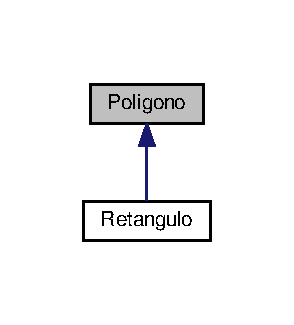
\includegraphics[width=141pt]{class_poligono__inherit__graph}
\end{center}
\end{figure}
\subsection*{Public Member Functions}
\begin{DoxyCompactItemize}
\item 
void \hyperlink{class_poligono_aa16b7ba7aaed5bdbef77862a69901823}{setn\+Vertices} (int n)
\begin{DoxyCompactList}\small\item\em setn\+Vertices insere vértices no \hyperlink{class_poligono}{Poligono} \end{DoxyCompactList}\item 
int \hyperlink{class_poligono_a0f63ca667ce8c15230353a5130baf3dd}{num\+Vet\+Pol} (void)
\begin{DoxyCompactList}\small\item\em num\+Vet\+Pol recupera a quantidade de vértices que foram inseridos no \hyperlink{class_poligono}{Poligono} \end{DoxyCompactList}\item 
void \hyperlink{class_poligono_a07656338edbd5bbd0b9bb7f4272717c1}{set\+Vet\+Pol} (int i, float x, float y)
\begin{DoxyCompactList}\small\item\em set\+Vet\+Pol altera os valores das coordenadas x e y de um vértice (\hyperlink{class_ponto}{Ponto}) do \hyperlink{class_poligono}{Poligono} \end{DoxyCompactList}\item 
void \hyperlink{class_poligono_a22bdea51dc2a5907b6f2f2dcf034c155}{add\+Pol} (int n)
\begin{DoxyCompactList}\small\item\em add\+Pol adiciona valores aos vértices do Polígono \end{DoxyCompactList}\item 
float \hyperlink{class_poligono_a5cc5994a3ec316c29b32c0f514167e88}{calc\+Area\+Pol} (void)
\begin{DoxyCompactList}\small\item\em calc\+Area\+Pol calcula a área de um \hyperlink{class_poligono}{Poligono} \end{DoxyCompactList}\item 
void \hyperlink{class_poligono_aa4948d6082b1cde7f7b683dacb88fde7}{translada\+Pol} (float a, float b)
\begin{DoxyCompactList}\small\item\em translada\+Pol translada um \hyperlink{class_poligono}{Poligono} \end{DoxyCompactList}\item 
void \hyperlink{class_poligono_a615deb0368ea28feb68d325c2d17e32f}{rotacionar\+Pol} (float angulo, float a, float b)
\begin{DoxyCompactList}\small\item\em rotacionar\+Pol rotaciona um \hyperlink{class_poligono}{Poligono} em torno de um \hyperlink{class_ponto}{Ponto} informado \end{DoxyCompactList}\item 
void \hyperlink{class_poligono_a21b124867ac9d4aa7e9a06fc0219b211}{imprime\+Pol} ()
\begin{DoxyCompactList}\small\item\em imprime\+Pol exibe um \hyperlink{class_poligono}{Poligono} \end{DoxyCompactList}\end{DoxyCompactItemize}


\subsection{Detailed Description}
A classe \hyperlink{class_poligono}{Poligono} representa polígonos convexos de até 100 vértices. 

\subsection{Member Function Documentation}
\index{Poligono@{Poligono}!add\+Pol@{add\+Pol}}
\index{add\+Pol@{add\+Pol}!Poligono@{Poligono}}
\subsubsection[{\texorpdfstring{add\+Pol(int n)}{addPol(int n)}}]{\setlength{\rightskip}{0pt plus 5cm}void Poligono\+::add\+Pol (
\begin{DoxyParamCaption}
\item[{int}]{n}
\end{DoxyParamCaption}
)}\hypertarget{class_poligono_a22bdea51dc2a5907b6f2f2dcf034c155}{}\label{class_poligono_a22bdea51dc2a5907b6f2f2dcf034c155}


add\+Pol adiciona valores aos vértices do Polígono 


\begin{DoxyParams}{Parameters}
{\em n} & é a quantidade de vértices a serem adicionados no \hyperlink{class_poligono}{Poligono} \\
\hline
\end{DoxyParams}
\index{Poligono@{Poligono}!calc\+Area\+Pol@{calc\+Area\+Pol}}
\index{calc\+Area\+Pol@{calc\+Area\+Pol}!Poligono@{Poligono}}
\subsubsection[{\texorpdfstring{calc\+Area\+Pol(void)}{calcAreaPol(void)}}]{\setlength{\rightskip}{0pt plus 5cm}float Poligono\+::calc\+Area\+Pol (
\begin{DoxyParamCaption}
\item[{void}]{}
\end{DoxyParamCaption}
)}\hypertarget{class_poligono_a5cc5994a3ec316c29b32c0f514167e88}{}\label{class_poligono_a5cc5994a3ec316c29b32c0f514167e88}


calc\+Area\+Pol calcula a área de um \hyperlink{class_poligono}{Poligono} 

\begin{DoxyReturn}{Returns}
valor da área do \hyperlink{class_poligono}{Poligono} 
\end{DoxyReturn}
\index{Poligono@{Poligono}!imprime\+Pol@{imprime\+Pol}}
\index{imprime\+Pol@{imprime\+Pol}!Poligono@{Poligono}}
\subsubsection[{\texorpdfstring{imprime\+Pol()}{imprimePol()}}]{\setlength{\rightskip}{0pt plus 5cm}void Poligono\+::imprime\+Pol (
\begin{DoxyParamCaption}
{}
\end{DoxyParamCaption}
)}\hypertarget{class_poligono_a21b124867ac9d4aa7e9a06fc0219b211}{}\label{class_poligono_a21b124867ac9d4aa7e9a06fc0219b211}


imprime\+Pol exibe um \hyperlink{class_poligono}{Poligono} 

\index{Poligono@{Poligono}!num\+Vet\+Pol@{num\+Vet\+Pol}}
\index{num\+Vet\+Pol@{num\+Vet\+Pol}!Poligono@{Poligono}}
\subsubsection[{\texorpdfstring{num\+Vet\+Pol(void)}{numVetPol(void)}}]{\setlength{\rightskip}{0pt plus 5cm}int Poligono\+::num\+Vet\+Pol (
\begin{DoxyParamCaption}
\item[{void}]{}
\end{DoxyParamCaption}
)}\hypertarget{class_poligono_a0f63ca667ce8c15230353a5130baf3dd}{}\label{class_poligono_a0f63ca667ce8c15230353a5130baf3dd}


num\+Vet\+Pol recupera a quantidade de vértices que foram inseridos no \hyperlink{class_poligono}{Poligono} 

\begin{DoxyReturn}{Returns}
valor com a quantidade de vértices inseridos 
\end{DoxyReturn}
\index{Poligono@{Poligono}!rotacionar\+Pol@{rotacionar\+Pol}}
\index{rotacionar\+Pol@{rotacionar\+Pol}!Poligono@{Poligono}}
\subsubsection[{\texorpdfstring{rotacionar\+Pol(float angulo, float a, float b)}{rotacionarPol(float angulo, float a, float b)}}]{\setlength{\rightskip}{0pt plus 5cm}void Poligono\+::rotacionar\+Pol (
\begin{DoxyParamCaption}
\item[{float}]{angulo, }
\item[{float}]{a, }
\item[{float}]{b}
\end{DoxyParamCaption}
)}\hypertarget{class_poligono_a615deb0368ea28feb68d325c2d17e32f}{}\label{class_poligono_a615deb0368ea28feb68d325c2d17e32f}


rotacionar\+Pol rotaciona um \hyperlink{class_poligono}{Poligono} em torno de um \hyperlink{class_ponto}{Ponto} informado 


\begin{DoxyParams}{Parameters}
{\em angulo} & é o ângulo de rotação a ser aplicado \\
\hline
{\em a} & é o valor da componente x do ponto de referência da rotacão \\
\hline
{\em b} & é o valor da componente y do ponto de referência da rotacao \\
\hline
\end{DoxyParams}
\index{Poligono@{Poligono}!setn\+Vertices@{setn\+Vertices}}
\index{setn\+Vertices@{setn\+Vertices}!Poligono@{Poligono}}
\subsubsection[{\texorpdfstring{setn\+Vertices(int n)}{setnVertices(int n)}}]{\setlength{\rightskip}{0pt plus 5cm}void Poligono\+::setn\+Vertices (
\begin{DoxyParamCaption}
\item[{int}]{n}
\end{DoxyParamCaption}
)}\hypertarget{class_poligono_aa16b7ba7aaed5bdbef77862a69901823}{}\label{class_poligono_aa16b7ba7aaed5bdbef77862a69901823}


setn\+Vertices insere vértices no \hyperlink{class_poligono}{Poligono} 


\begin{DoxyParams}{Parameters}
{\em n} & é o parâmetro que determina a quantidade de vértices do \hyperlink{class_poligono}{Poligono} \\
\hline
\end{DoxyParams}
\index{Poligono@{Poligono}!set\+Vet\+Pol@{set\+Vet\+Pol}}
\index{set\+Vet\+Pol@{set\+Vet\+Pol}!Poligono@{Poligono}}
\subsubsection[{\texorpdfstring{set\+Vet\+Pol(int i, float x, float y)}{setVetPol(int i, float x, float y)}}]{\setlength{\rightskip}{0pt plus 5cm}void Poligono\+::set\+Vet\+Pol (
\begin{DoxyParamCaption}
\item[{int}]{i, }
\item[{float}]{x, }
\item[{float}]{y}
\end{DoxyParamCaption}
)}\hypertarget{class_poligono_a07656338edbd5bbd0b9bb7f4272717c1}{}\label{class_poligono_a07656338edbd5bbd0b9bb7f4272717c1}


set\+Vet\+Pol altera os valores das coordenadas x e y de um vértice (\hyperlink{class_ponto}{Ponto}) do \hyperlink{class_poligono}{Poligono} 


\begin{DoxyParams}{Parameters}
{\em i} & é o parâmetro que indica o vértice (\hyperlink{class_ponto}{Ponto}) a ser alterado \\
\hline
{\em x} & é o valor a ser alterado na coordenada x do vértice \\
\hline
{\em y} & é o valor a ser alterado na coordenada y do vértice \\
\hline
\end{DoxyParams}
\index{Poligono@{Poligono}!translada\+Pol@{translada\+Pol}}
\index{translada\+Pol@{translada\+Pol}!Poligono@{Poligono}}
\subsubsection[{\texorpdfstring{translada\+Pol(float a, float b)}{transladaPol(float a, float b)}}]{\setlength{\rightskip}{0pt plus 5cm}void Poligono\+::translada\+Pol (
\begin{DoxyParamCaption}
\item[{float}]{a, }
\item[{float}]{b}
\end{DoxyParamCaption}
)}\hypertarget{class_poligono_aa4948d6082b1cde7f7b683dacb88fde7}{}\label{class_poligono_aa4948d6082b1cde7f7b683dacb88fde7}


translada\+Pol translada um \hyperlink{class_poligono}{Poligono} 


\begin{DoxyParams}{Parameters}
{\em a} & é o valor a ser transladado pelo \hyperlink{class_poligono}{Poligono} no eixo x \\
\hline
{\em b} & é o valor a ser transladado pelo \hyperlink{class_poligono}{Poligono} no eixo y \\
\hline
\end{DoxyParams}


The documentation for this class was generated from the following files\+:\begin{DoxyCompactItemize}
\item 
\hyperlink{poligono_8h}{poligono.\+h}\item 
\hyperlink{poligono_8cpp}{poligono.\+cpp}\end{DoxyCompactItemize}

\hypertarget{class_ponto}{}\section{Ponto Class Reference}
\label{class_ponto}\index{Ponto@{Ponto}}


A classe \hyperlink{class_ponto}{Ponto} representa pontos no espaço bidimensional.  




{\ttfamily \#include $<$ponto.\+h$>$}

\subsection*{Public Member Functions}
\begin{DoxyCompactItemize}
\item 
\hyperlink{class_ponto_a5a157b4f3dc28842de40f505666f8899}{Ponto} (float \+\_\+x=0, float \+\_\+y=0)
\begin{DoxyCompactList}\small\item\em \hyperlink{class_ponto}{Ponto} é o construtor da classe \hyperlink{class_ponto}{Ponto}. \end{DoxyCompactList}\item 
void \hyperlink{class_ponto_a22129ad4dbf8019c479021d70a9f6774}{setX} (float \+\_\+x)
\begin{DoxyCompactList}\small\item\em setX altera o valor da coordenada x de um objeto da classe \hyperlink{class_ponto}{Ponto} \end{DoxyCompactList}\item 
void \hyperlink{class_ponto_a2d9e5b9fade9d3f3f21122a2dc2f5e11}{setY} (float \+\_\+y)
\begin{DoxyCompactList}\small\item\em setY altera o valor da coordenada y de um objeto da classe \hyperlink{class_ponto}{Ponto} \end{DoxyCompactList}\item 
float \hyperlink{class_ponto_a81256752897090e5424fdabb992407b5}{getX} (void)
\begin{DoxyCompactList}\small\item\em getX recupera o valor da coordenada x de um objeto da classe \hyperlink{class_ponto}{Ponto} \end{DoxyCompactList}\item 
float \hyperlink{class_ponto_a554a249ab828ccfd6173380a4d81010f}{getY} (void)
\begin{DoxyCompactList}\small\item\em getY recupera o valor da coordenada y de um objeto da classe \hyperlink{class_ponto}{Ponto} \end{DoxyCompactList}\item 
void \hyperlink{class_ponto_a827488219a7da184d440f687cec49ce6}{set\+XY} (float \+\_\+x, float \+\_\+y)
\begin{DoxyCompactList}\small\item\em set\+XY altera os valores das coordenadas x e y de um objeto da classe \hyperlink{class_ponto}{Ponto} \end{DoxyCompactList}\item 
void \hyperlink{class_ponto_ad4eb84742e5823fcf4b7fe6f7b1202ed}{add} (\hyperlink{class_ponto}{Ponto} p)
\begin{DoxyCompactList}\small\item\em add realiza a operação de soma de 2 pontos \end{DoxyCompactList}\item 
void \hyperlink{class_ponto_a8863be0ba572c78b0133a6d49993df1b}{sub} (\hyperlink{class_ponto}{Ponto} p)
\begin{DoxyCompactList}\small\item\em sub realiza a operação de subtração de 2 pontos \end{DoxyCompactList}\item 
float \hyperlink{class_ponto_acf5167ec08bdd5fbf71bc6a4f1438edc}{norma} (void)
\begin{DoxyCompactList}\small\item\em norma calcula a norma de um ponto \end{DoxyCompactList}\item 
void \hyperlink{class_ponto_a96a4395204ec010814e67d20705e630f}{translada} (float a, float b)
\begin{DoxyCompactList}\small\item\em translada é um método que translada um objeto da classe \hyperlink{class_ponto}{Ponto} \end{DoxyCompactList}\item 
void \hyperlink{class_ponto_a527d46ce0fc24f112ead68980e52c2ca}{imprime} (void)
\begin{DoxyCompactList}\small\item\em imprime exibe um objeto da classe \hyperlink{class_ponto}{Ponto} \end{DoxyCompactList}\end{DoxyCompactItemize}


\subsection{Detailed Description}
A classe \hyperlink{class_ponto}{Ponto} representa pontos no espaço bidimensional. 

\subsection{Constructor \& Destructor Documentation}
\index{Ponto@{Ponto}!Ponto@{Ponto}}
\index{Ponto@{Ponto}!Ponto@{Ponto}}
\subsubsection[{\texorpdfstring{Ponto(float \+\_\+x=0, float \+\_\+y=0)}{Ponto(float _x=0, float _y=0)}}]{\setlength{\rightskip}{0pt plus 5cm}Ponto\+::\+Ponto (
\begin{DoxyParamCaption}
\item[{float}]{\+\_\+x = {\ttfamily 0}, }
\item[{float}]{\+\_\+y = {\ttfamily 0}}
\end{DoxyParamCaption}
)}\hypertarget{class_ponto_a5a157b4f3dc28842de40f505666f8899}{}\label{class_ponto_a5a157b4f3dc28842de40f505666f8899}


\hyperlink{class_ponto}{Ponto} é o construtor da classe \hyperlink{class_ponto}{Ponto}. 


\begin{DoxyParams}{Parameters}
{\em \+\_\+x} & é o parâmetro que define a coordenada x de um objeto da classe \hyperlink{class_ponto}{Ponto} \\
\hline
{\em \+\_\+y} & é o parâmetro que define a coordenada y de um objeto da classe \hyperlink{class_ponto}{Ponto}\\
\hline
\end{DoxyParams}
se um objeto dessa classe for criado sem a passagem de parâmetros para o construtor, o objeto será um \hyperlink{class_ponto}{Ponto} de coordenada (0,0) 

\subsection{Member Function Documentation}
\index{Ponto@{Ponto}!add@{add}}
\index{add@{add}!Ponto@{Ponto}}
\subsubsection[{\texorpdfstring{add(\+Ponto p)}{add(Ponto p)}}]{\setlength{\rightskip}{0pt plus 5cm}void Ponto\+::add (
\begin{DoxyParamCaption}
\item[{{\bf Ponto}}]{p}
\end{DoxyParamCaption}
)}\hypertarget{class_ponto_ad4eb84742e5823fcf4b7fe6f7b1202ed}{}\label{class_ponto_ad4eb84742e5823fcf4b7fe6f7b1202ed}


add realiza a operação de soma de 2 pontos 


\begin{DoxyParams}{Parameters}
{\em p} & é o objeto do tipo \hyperlink{class_ponto}{Ponto} a ser somado \\
\hline
\end{DoxyParams}
\index{Ponto@{Ponto}!getX@{getX}}
\index{getX@{getX}!Ponto@{Ponto}}
\subsubsection[{\texorpdfstring{get\+X(void)}{getX(void)}}]{\setlength{\rightskip}{0pt plus 5cm}float Ponto\+::getX (
\begin{DoxyParamCaption}
\item[{void}]{}
\end{DoxyParamCaption}
)}\hypertarget{class_ponto_a81256752897090e5424fdabb992407b5}{}\label{class_ponto_a81256752897090e5424fdabb992407b5}


getX recupera o valor da coordenada x de um objeto da classe \hyperlink{class_ponto}{Ponto} 

\begin{DoxyReturn}{Returns}
valor da coordenada x da classe \hyperlink{class_ponto}{Ponto} 
\end{DoxyReturn}
\index{Ponto@{Ponto}!getY@{getY}}
\index{getY@{getY}!Ponto@{Ponto}}
\subsubsection[{\texorpdfstring{get\+Y(void)}{getY(void)}}]{\setlength{\rightskip}{0pt plus 5cm}float Ponto\+::getY (
\begin{DoxyParamCaption}
\item[{void}]{}
\end{DoxyParamCaption}
)}\hypertarget{class_ponto_a554a249ab828ccfd6173380a4d81010f}{}\label{class_ponto_a554a249ab828ccfd6173380a4d81010f}


getY recupera o valor da coordenada y de um objeto da classe \hyperlink{class_ponto}{Ponto} 

\begin{DoxyReturn}{Returns}
valor da coordenada y da classe \hyperlink{class_ponto}{Ponto} 
\end{DoxyReturn}
\index{Ponto@{Ponto}!imprime@{imprime}}
\index{imprime@{imprime}!Ponto@{Ponto}}
\subsubsection[{\texorpdfstring{imprime(void)}{imprime(void)}}]{\setlength{\rightskip}{0pt plus 5cm}void Ponto\+::imprime (
\begin{DoxyParamCaption}
\item[{void}]{}
\end{DoxyParamCaption}
)}\hypertarget{class_ponto_a527d46ce0fc24f112ead68980e52c2ca}{}\label{class_ponto_a527d46ce0fc24f112ead68980e52c2ca}


imprime exibe um objeto da classe \hyperlink{class_ponto}{Ponto} 

\index{Ponto@{Ponto}!norma@{norma}}
\index{norma@{norma}!Ponto@{Ponto}}
\subsubsection[{\texorpdfstring{norma(void)}{norma(void)}}]{\setlength{\rightskip}{0pt plus 5cm}float Ponto\+::norma (
\begin{DoxyParamCaption}
\item[{void}]{}
\end{DoxyParamCaption}
)}\hypertarget{class_ponto_acf5167ec08bdd5fbf71bc6a4f1438edc}{}\label{class_ponto_acf5167ec08bdd5fbf71bc6a4f1438edc}


norma calcula a norma de um ponto 

\begin{DoxyReturn}{Returns}
o valor da norma do ponto. 
\end{DoxyReturn}
\index{Ponto@{Ponto}!setX@{setX}}
\index{setX@{setX}!Ponto@{Ponto}}
\subsubsection[{\texorpdfstring{set\+X(float \+\_\+x)}{setX(float _x)}}]{\setlength{\rightskip}{0pt plus 5cm}void Ponto\+::setX (
\begin{DoxyParamCaption}
\item[{float}]{\+\_\+x}
\end{DoxyParamCaption}
)}\hypertarget{class_ponto_a22129ad4dbf8019c479021d70a9f6774}{}\label{class_ponto_a22129ad4dbf8019c479021d70a9f6774}


setX altera o valor da coordenada x de um objeto da classe \hyperlink{class_ponto}{Ponto} 


\begin{DoxyParams}{Parameters}
{\em \+\_\+x} & é o parâmetro para o valor a ser alterado na coordenada x. \\
\hline
\end{DoxyParams}
\index{Ponto@{Ponto}!set\+XY@{set\+XY}}
\index{set\+XY@{set\+XY}!Ponto@{Ponto}}
\subsubsection[{\texorpdfstring{set\+X\+Y(float \+\_\+x, float \+\_\+y)}{setXY(float _x, float _y)}}]{\setlength{\rightskip}{0pt plus 5cm}void Ponto\+::set\+XY (
\begin{DoxyParamCaption}
\item[{float}]{\+\_\+x, }
\item[{float}]{\+\_\+y}
\end{DoxyParamCaption}
)}\hypertarget{class_ponto_a827488219a7da184d440f687cec49ce6}{}\label{class_ponto_a827488219a7da184d440f687cec49ce6}


set\+XY altera os valores das coordenadas x e y de um objeto da classe \hyperlink{class_ponto}{Ponto} 


\begin{DoxyParams}{Parameters}
{\em \+\_\+x} & é o parâmetro para o valor a ser alterado na coordenada x. \\
\hline
{\em \+\_\+y} & é o parâmetro para o valor a ser alterado na coordenada y. \\
\hline
\end{DoxyParams}
\index{Ponto@{Ponto}!setY@{setY}}
\index{setY@{setY}!Ponto@{Ponto}}
\subsubsection[{\texorpdfstring{set\+Y(float \+\_\+y)}{setY(float _y)}}]{\setlength{\rightskip}{0pt plus 5cm}void Ponto\+::setY (
\begin{DoxyParamCaption}
\item[{float}]{\+\_\+y}
\end{DoxyParamCaption}
)}\hypertarget{class_ponto_a2d9e5b9fade9d3f3f21122a2dc2f5e11}{}\label{class_ponto_a2d9e5b9fade9d3f3f21122a2dc2f5e11}


setY altera o valor da coordenada y de um objeto da classe \hyperlink{class_ponto}{Ponto} 


\begin{DoxyParams}{Parameters}
{\em \+\_\+y} & é o parâmetro para o valor a ser alterado na coordenada y. \\
\hline
\end{DoxyParams}
\index{Ponto@{Ponto}!sub@{sub}}
\index{sub@{sub}!Ponto@{Ponto}}
\subsubsection[{\texorpdfstring{sub(\+Ponto p)}{sub(Ponto p)}}]{\setlength{\rightskip}{0pt plus 5cm}void Ponto\+::sub (
\begin{DoxyParamCaption}
\item[{{\bf Ponto}}]{p}
\end{DoxyParamCaption}
)}\hypertarget{class_ponto_a8863be0ba572c78b0133a6d49993df1b}{}\label{class_ponto_a8863be0ba572c78b0133a6d49993df1b}


sub realiza a operação de subtração de 2 pontos 


\begin{DoxyParams}{Parameters}
{\em p} & é o objeto do tipo \hyperlink{class_ponto}{Ponto} a ser subtraído \\
\hline
\end{DoxyParams}
\index{Ponto@{Ponto}!translada@{translada}}
\index{translada@{translada}!Ponto@{Ponto}}
\subsubsection[{\texorpdfstring{translada(float a, float b)}{translada(float a, float b)}}]{\setlength{\rightskip}{0pt plus 5cm}void Ponto\+::translada (
\begin{DoxyParamCaption}
\item[{float}]{a, }
\item[{float}]{b}
\end{DoxyParamCaption}
)}\hypertarget{class_ponto_a96a4395204ec010814e67d20705e630f}{}\label{class_ponto_a96a4395204ec010814e67d20705e630f}


translada é um método que translada um objeto da classe \hyperlink{class_ponto}{Ponto} 


\begin{DoxyParams}{Parameters}
{\em a} & é o valor a ser transladado na coordenada x. \\
\hline
{\em b} & é o valor a ser transladado na coordenada y. \\
\hline
\end{DoxyParams}


The documentation for this class was generated from the following files\+:\begin{DoxyCompactItemize}
\item 
\hyperlink{ponto_8h}{ponto.\+h}\item 
\hyperlink{ponto_8cpp}{ponto.\+cpp}\end{DoxyCompactItemize}

\hypertarget{class_retangulo}{}\section{Retangulo Class Reference}
\label{class_retangulo}\index{Retangulo@{Retangulo}}


A classe \hyperlink{class_retangulo}{Retangulo} cria um objeto do tipo \hyperlink{class_retangulo}{Retangulo} que pode ser desenhada numa \hyperlink{class_screen}{Screen}.  




{\ttfamily \#include $<$retangulo.\+h$>$}



Inheritance diagram for Retangulo\+:
\nopagebreak
\begin{figure}[H]
\begin{center}
\leavevmode
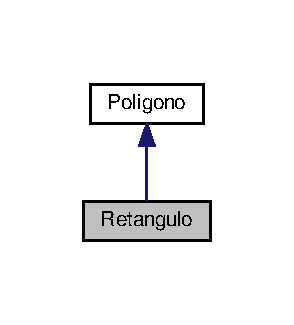
\includegraphics[width=174pt]{class_retangulo__inherit__graph}
\end{center}
\end{figure}


Collaboration diagram for Retangulo\+:
\nopagebreak
\begin{figure}[H]
\begin{center}
\leavevmode
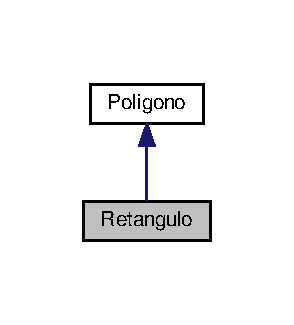
\includegraphics[width=174pt]{class_retangulo__coll__graph}
\end{center}
\end{figure}
\subsection*{Public Member Functions}
\begin{DoxyCompactItemize}
\item 
\hyperlink{class_retangulo_ad1646092a00ba28fcaa8390ce366f3b7}{Retangulo} (int \+\_\+x0=0, int \+\_\+y0=0, int \+\_\+l=0, int \+\_\+a=0, int \+\_\+fillmode=0, char \+\_\+brush=\textquotesingle{}$\ast$\textquotesingle{})
\begin{DoxyCompactList}\small\item\em \hyperlink{class_retangulo}{Retangulo} é o construtor da classe \hyperlink{class_retangulo}{Retangulo}. \end{DoxyCompactList}\item 
void \hyperlink{class_retangulo_ac088dd6d3f4f3d3f80363a868c2e74f1}{draw} (\hyperlink{class_screen}{Screen} \&t)
\begin{DoxyCompactList}\small\item\em draw desenha um \hyperlink{class_retangulo}{Retangulo} numa tela \end{DoxyCompactList}\end{DoxyCompactItemize}


\subsection{Detailed Description}
A classe \hyperlink{class_retangulo}{Retangulo} cria um objeto do tipo \hyperlink{class_retangulo}{Retangulo} que pode ser desenhada numa \hyperlink{class_screen}{Screen}. 

Esta classe extende a classe \hyperlink{class_figura_geometrica}{Figura\+Geometrica} 

\subsection{Constructor \& Destructor Documentation}
\index{Retangulo@{Retangulo}!Retangulo@{Retangulo}}
\index{Retangulo@{Retangulo}!Retangulo@{Retangulo}}
\subsubsection[{\texorpdfstring{Retangulo(int \+\_\+x0=0, int \+\_\+y0=0, int \+\_\+l=0, int \+\_\+a=0, int \+\_\+fillmode=0, char \+\_\+brush=\textquotesingle{}$\ast$\textquotesingle{})}{Retangulo(int _x0=0, int _y0=0, int _l=0, int _a=0, int _fillmode=0, char _brush='*')}}]{\setlength{\rightskip}{0pt plus 5cm}Retangulo\+::\+Retangulo (
\begin{DoxyParamCaption}
\item[{int}]{\+\_\+x0 = {\ttfamily 0}, }
\item[{int}]{\+\_\+y0 = {\ttfamily 0}, }
\item[{int}]{\+\_\+l = {\ttfamily 0}, }
\item[{int}]{\+\_\+a = {\ttfamily 0}, }
\item[{int}]{\+\_\+fillmode = {\ttfamily 0}, }
\item[{char}]{\+\_\+brush = {\ttfamily \textquotesingle{}$\ast$\textquotesingle{}}}
\end{DoxyParamCaption}
)}\hypertarget{class_retangulo_ad1646092a00ba28fcaa8390ce366f3b7}{}\label{class_retangulo_ad1646092a00ba28fcaa8390ce366f3b7}


\hyperlink{class_retangulo}{Retangulo} é o construtor da classe \hyperlink{class_retangulo}{Retangulo}. 


\begin{DoxyParams}{Parameters}
{\em \+\_\+x0} & é o valor da coordenada x do ponto superior esquerdo do \hyperlink{class_retangulo}{Retangulo} \\
\hline
{\em \+\_\+y0} & é o valor da coordenada y do ponto superior esquerdo do \hyperlink{class_retangulo}{Retangulo} \\
\hline
{\em \+\_\+l} & é o valor da largura do \hyperlink{class_retangulo}{Retangulo} \\
\hline
{\em \+\_\+a} & é o valor da altura do \hyperlink{class_retangulo}{Retangulo} \\
\hline
{\em \+\_\+fillmode} & indica se o \hyperlink{class_retangulo}{Retangulo} deve ser preenchido ou não \\
\hline
{\em \+\_\+brush} & indica o caractere a ser usado para desenhar o \hyperlink{class_retangulo}{Retangulo} uma tela \\
\hline
\end{DoxyParams}


\subsection{Member Function Documentation}
\index{Retangulo@{Retangulo}!draw@{draw}}
\index{draw@{draw}!Retangulo@{Retangulo}}
\subsubsection[{\texorpdfstring{draw(\+Screen \&t)}{draw(Screen &t)}}]{\setlength{\rightskip}{0pt plus 5cm}void Retangulo\+::draw (
\begin{DoxyParamCaption}
\item[{{\bf Screen} \&}]{t}
\end{DoxyParamCaption}
)\hspace{0.3cm}{\ttfamily [virtual]}}\hypertarget{class_retangulo_ac088dd6d3f4f3d3f80363a868c2e74f1}{}\label{class_retangulo_ac088dd6d3f4f3d3f80363a868c2e74f1}


draw desenha um \hyperlink{class_retangulo}{Retangulo} numa tela 


\begin{DoxyParams}{Parameters}
{\em t} & é a tela na qual se deseja desenhar \\
\hline
\end{DoxyParams}


Implements \hyperlink{class_figura_geometrica_a8ee8dedc060b6059a805ea091aef2c41}{Figura\+Geometrica}.



The documentation for this class was generated from the following files\+:\begin{DoxyCompactItemize}
\item 
\hyperlink{retangulo_8h}{retangulo.\+h}\item 
\hyperlink{retangulo_8cpp}{retangulo.\+cpp}\end{DoxyCompactItemize}

\chapter{File Documentation}
\hypertarget{main_8cpp}{}\section{Qt\+Tcp\+Server/main.cpp File Reference}
\label{main_8cpp}\index{Qt\+Tcp\+Server/main.\+cpp@{Qt\+Tcp\+Server/main.\+cpp}}
{\ttfamily \#include \char`\"{}mainwindow.\+h\char`\"{}}\\*
{\ttfamily \#include $<$Q\+Application$>$}\\*
Include dependency graph for main.\+cpp\+:
\nopagebreak
\begin{figure}[H]
\begin{center}
\leavevmode
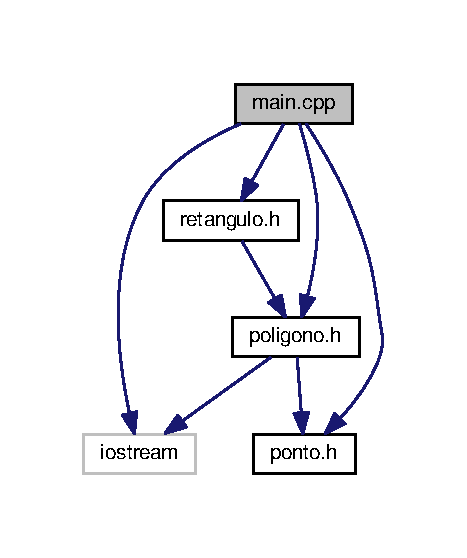
\includegraphics[width=350pt]{main_8cpp__incl}
\end{center}
\end{figure}
\subsection*{Functions}
\begin{DoxyCompactItemize}
\item 
int \hyperlink{main_8cpp_a0ddf1224851353fc92bfbff6f499fa97}{main} (int argc, char $\ast$argv\mbox{[}$\,$\mbox{]})
\end{DoxyCompactItemize}


\subsection{Function Documentation}
\index{main.\+cpp@{main.\+cpp}!main@{main}}
\index{main@{main}!main.\+cpp@{main.\+cpp}}
\subsubsection[{\texorpdfstring{main(int argc, char $\ast$argv[])}{main(int argc, char *argv[])}}]{\setlength{\rightskip}{0pt plus 5cm}int main (
\begin{DoxyParamCaption}
\item[{int}]{argc, }
\item[{char $\ast$}]{argv\mbox{[}$\,$\mbox{]}}
\end{DoxyParamCaption}
)}\hypertarget{main_8cpp_a0ddf1224851353fc92bfbff6f499fa97}{}\label{main_8cpp_a0ddf1224851353fc92bfbff6f499fa97}

\hypertarget{poligono_8cpp}{}\section{poligono.\+cpp File Reference}
\label{poligono_8cpp}\index{poligono.\+cpp@{poligono.\+cpp}}
{\ttfamily \#include \char`\"{}poligono.\+h\char`\"{}}\\*
{\ttfamily \#include $<$cmath$>$}\\*
Include dependency graph for poligono.\+cpp\+:\nopagebreak
\begin{figure}[H]
\begin{center}
\leavevmode
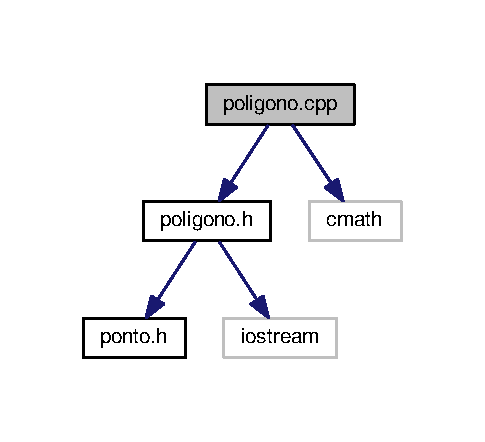
\includegraphics[width=233pt]{poligono_8cpp__incl}
\end{center}
\end{figure}
\subsection*{Macros}
\begin{DoxyCompactItemize}
\item 
\#define \hyperlink{poligono_8cpp_a598a3330b3c21701223ee0ca14316eca}{PI}~3.\+14159265
\end{DoxyCompactItemize}


\subsection{Macro Definition Documentation}
\index{poligono.\+cpp@{poligono.\+cpp}!PI@{PI}}
\index{PI@{PI}!poligono.\+cpp@{poligono.\+cpp}}
\subsubsection[{\texorpdfstring{PI}{PI}}]{\setlength{\rightskip}{0pt plus 5cm}\#define PI~3.\+14159265}\hypertarget{poligono_8cpp_a598a3330b3c21701223ee0ca14316eca}{}\label{poligono_8cpp_a598a3330b3c21701223ee0ca14316eca}

\hypertarget{poligono_8h}{}\section{poligono.\+h File Reference}
\label{poligono_8h}\index{poligono.\+h@{poligono.\+h}}
{\ttfamily \#include \char`\"{}ponto.\+h\char`\"{}}\\*
{\ttfamily \#include $<$iostream$>$}\\*
Include dependency graph for poligono.\+h\+:\nopagebreak
\begin{figure}[H]
\begin{center}
\leavevmode
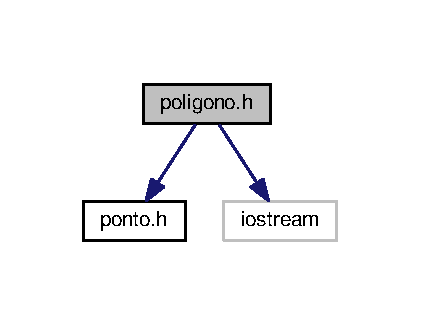
\includegraphics[width=202pt]{poligono_8h__incl}
\end{center}
\end{figure}
This graph shows which files directly or indirectly include this file\+:\nopagebreak
\begin{figure}[H]
\begin{center}
\leavevmode
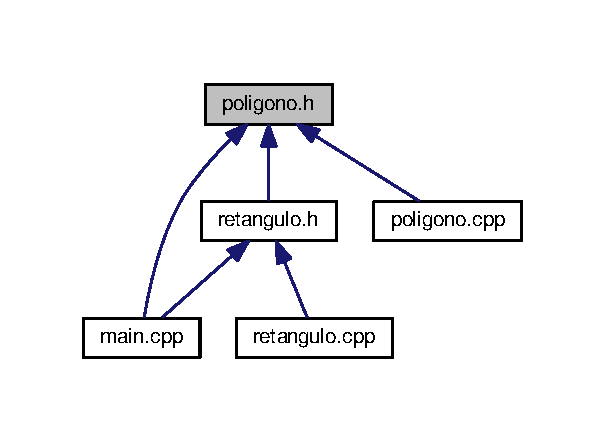
\includegraphics[width=291pt]{poligono_8h__dep__incl}
\end{center}
\end{figure}
\subsection*{Classes}
\begin{DoxyCompactItemize}
\item 
class \hyperlink{class_poligono}{Poligono}
\end{DoxyCompactItemize}
\subsection*{Macros}
\begin{DoxyCompactItemize}
\item 
\#define \hyperlink{poligono_8h_a0240ac851181b84ac374872dc5434ee4}{N}~100
\end{DoxyCompactItemize}


\subsection{Macro Definition Documentation}
\index{poligono.\+h@{poligono.\+h}!N@{N}}
\index{N@{N}!poligono.\+h@{poligono.\+h}}
\subsubsection[{\texorpdfstring{N}{N}}]{\setlength{\rightskip}{0pt plus 5cm}\#define N~100}\hypertarget{poligono_8h_a0240ac851181b84ac374872dc5434ee4}{}\label{poligono_8h_a0240ac851181b84ac374872dc5434ee4}

\hypertarget{ponto_8cpp}{}\section{ponto.\+cpp File Reference}
\label{ponto_8cpp}\index{ponto.\+cpp@{ponto.\+cpp}}
{\ttfamily \#include \char`\"{}ponto.\+h\char`\"{}}\\*
{\ttfamily \#include $<$iostream$>$}\\*
{\ttfamily \#include $<$cmath$>$}\\*
Include dependency graph for ponto.\+cpp\+:\nopagebreak
\begin{figure}[H]
\begin{center}
\leavevmode
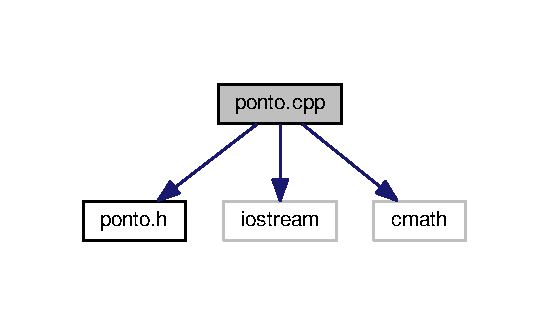
\includegraphics[width=264pt]{ponto_8cpp__incl}
\end{center}
\end{figure}

\hypertarget{ponto_8h}{}\section{ponto.\+h File Reference}
\label{ponto_8h}\index{ponto.\+h@{ponto.\+h}}
This graph shows which files directly or indirectly include this file\+:\nopagebreak
\begin{figure}[H]
\begin{center}
\leavevmode
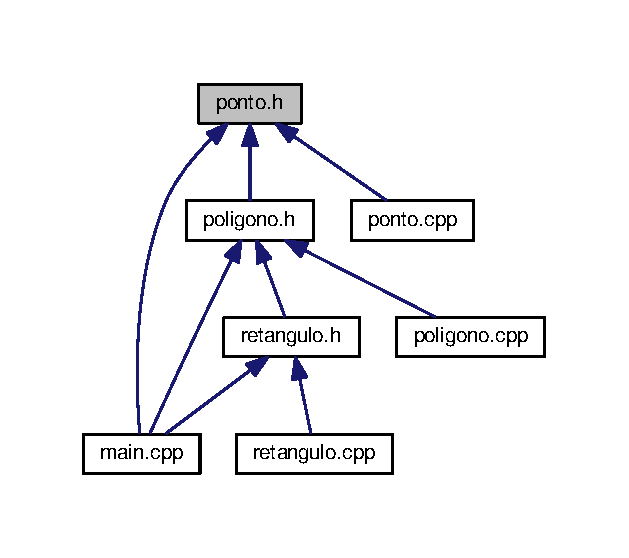
\includegraphics[width=302pt]{ponto_8h__dep__incl}
\end{center}
\end{figure}
\subsection*{Classes}
\begin{DoxyCompactItemize}
\item 
class \hyperlink{class_ponto}{Ponto}
\begin{DoxyCompactList}\small\item\em A classe \hyperlink{class_ponto}{Ponto} representa pontos no espaço bidimensional. \end{DoxyCompactList}\end{DoxyCompactItemize}

\hypertarget{retangulo_8cpp}{}\section{retangulo.\+cpp File Reference}
\label{retangulo_8cpp}\index{retangulo.\+cpp@{retangulo.\+cpp}}
{\ttfamily \#include \char`\"{}retangulo.\+h\char`\"{}}\\*
Include dependency graph for retangulo.\+cpp\+:
\nopagebreak
\begin{figure}[H]
\begin{center}
\leavevmode
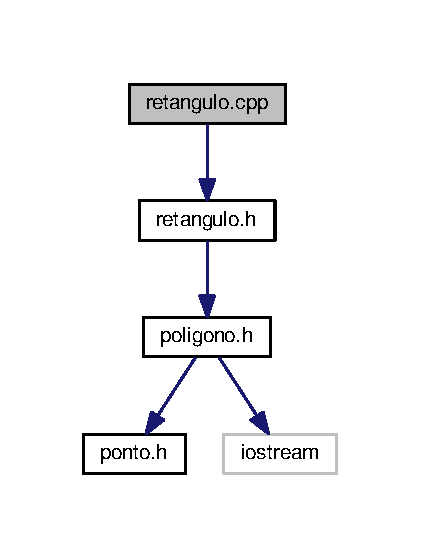
\includegraphics[width=266pt]{retangulo_8cpp__incl}
\end{center}
\end{figure}

\hypertarget{retangulo_8h}{}\section{retangulo.\+h File Reference}
\label{retangulo_8h}\index{retangulo.\+h@{retangulo.\+h}}
{\ttfamily \#include \char`\"{}poligono.\+h\char`\"{}}\\*
Include dependency graph for retangulo.\+h\+:\nopagebreak
\begin{figure}[H]
\begin{center}
\leavevmode
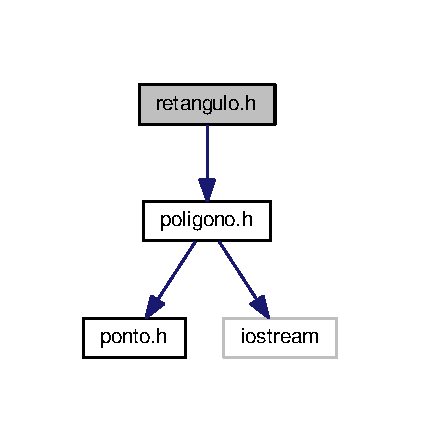
\includegraphics[width=202pt]{retangulo_8h__incl}
\end{center}
\end{figure}
This graph shows which files directly or indirectly include this file\+:\nopagebreak
\begin{figure}[H]
\begin{center}
\leavevmode
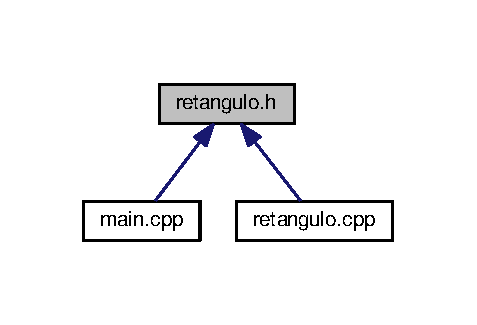
\includegraphics[width=229pt]{retangulo_8h__dep__incl}
\end{center}
\end{figure}
\subsection*{Classes}
\begin{DoxyCompactItemize}
\item 
class \hyperlink{class_retangulo}{Retangulo}
\begin{DoxyCompactList}\small\item\em A classe \hyperlink{class_retangulo}{Retangulo} é uma subclasse da classe \hyperlink{class_poligono}{Poligono} que representa retângulos. \end{DoxyCompactList}\end{DoxyCompactItemize}

%--- End generated contents ---

% Index
\backmatter
\newpage
\phantomsection
\clearemptydoublepage
\addcontentsline{toc}{chapter}{Index}
\printindex

\end{document}
